% G07 - ECOM060 - Fase 2, Entrega 02: equivalente eletrico no TyphoonSim
% Compilar com: xelatex relatorio.tex (duas vezes)
\documentclass[10pt,a4paper]{article}
\usepackage[margin=1.6cm,top=1.4cm,bottom=1.6cm]{geometry}
\usepackage{fontspec}
\setmainfont{TeX Gyre Termes}
\usepackage{amsmath,amssymb}
\usepackage{graphicx,booktabs,tabularx,multirow,array,xcolor}
\usepackage[font=small,labelfont=bf,labelsep=period]{caption}
\usepackage{enumitem}
\usepackage{newunicodechar}
\usepackage{placeins}
\usepackage{fancyvrb}
\newunicodechar{Ω}{\ensuremath{\Omega}}
\newunicodechar{→}{\ensuremath{\to}}
\newunicodechar{×}{\ensuremath{\times}}
\newunicodechar{·}{\ensuremath{\cdot}}
\newunicodechar{≤}{\ensuremath{\le}}
\newunicodechar{°}{\ensuremath{^\circ}}
\usepackage[hidelinks]{hyperref}
\renewcommand{\figurename}{Figura}
\renewcommand{\tablename}{Tabela}
\renewcommand{\refname}{Referências}
\setlist{nosep,leftmargin=*}
\setlength{\parskip}{2pt}
\newcolumntype{Y}{>{\raggedright\arraybackslash}X}
\newcommand{\fonteEq}{VHIL/HIL SCADA (Capture, 50 kS/s) nos ensaios de R3 (Fig.~\ref{fig:val} e Tab.~\ref{tab:val}); malha fechada original e Fig.~\ref{fig:corr}: TyphoonSim e netlist do \texttt{.tse}}

\makeatletter\let\inputtab\@@input\makeatother
\newcommand{\R}[1]{\FloatBarrier\par\medskip\noindent{\large\bfseries #1}\par\smallskip}

\emergencystretch=3em\sloppy
\begin{document}
\begin{center}
{\Large\bfseries Equivalente elétrico no TyphoonSim: motor BLDC MOONS' R42BLD30L3}\\[2pt]
Grupo G07 — Fase 2, Entrega 02 — ECOM060 Instrumentação Eletrônica (UFAL, 2026.2)\\[4pt]
\begin{tabular}{ll}\toprule Nome completo & Matrícula\\\midrule
Nícolas De Almeida Souza & 23111883\\ Lucas Momesso Alves & 22112804\\ Cláudio Henrique da Costa Santos & 20211850\\\bottomrule\end{tabular}
\end{center}

\R{Pendências da Entrega 01 e sistema}
O aval da Entrega 01 pediu (i) uma imagem real do sistema e (ii) uma descrição mais precisa de como a simulação foi feita. O grupo não dispõe do motor físico; a Fig.~\ref{fig:foto} mostra o sistema completo como foi implementado e executado no Typhoon; a seção ``Método de simulação'' e a Tab.~\ref{tab:metodo} descrevem, para a E01 e para esta entrega, o modelo, o integrador, o passo, as taxas de amostragem e a origem de cada curva.

\begin{figure}[!htbp]\centering
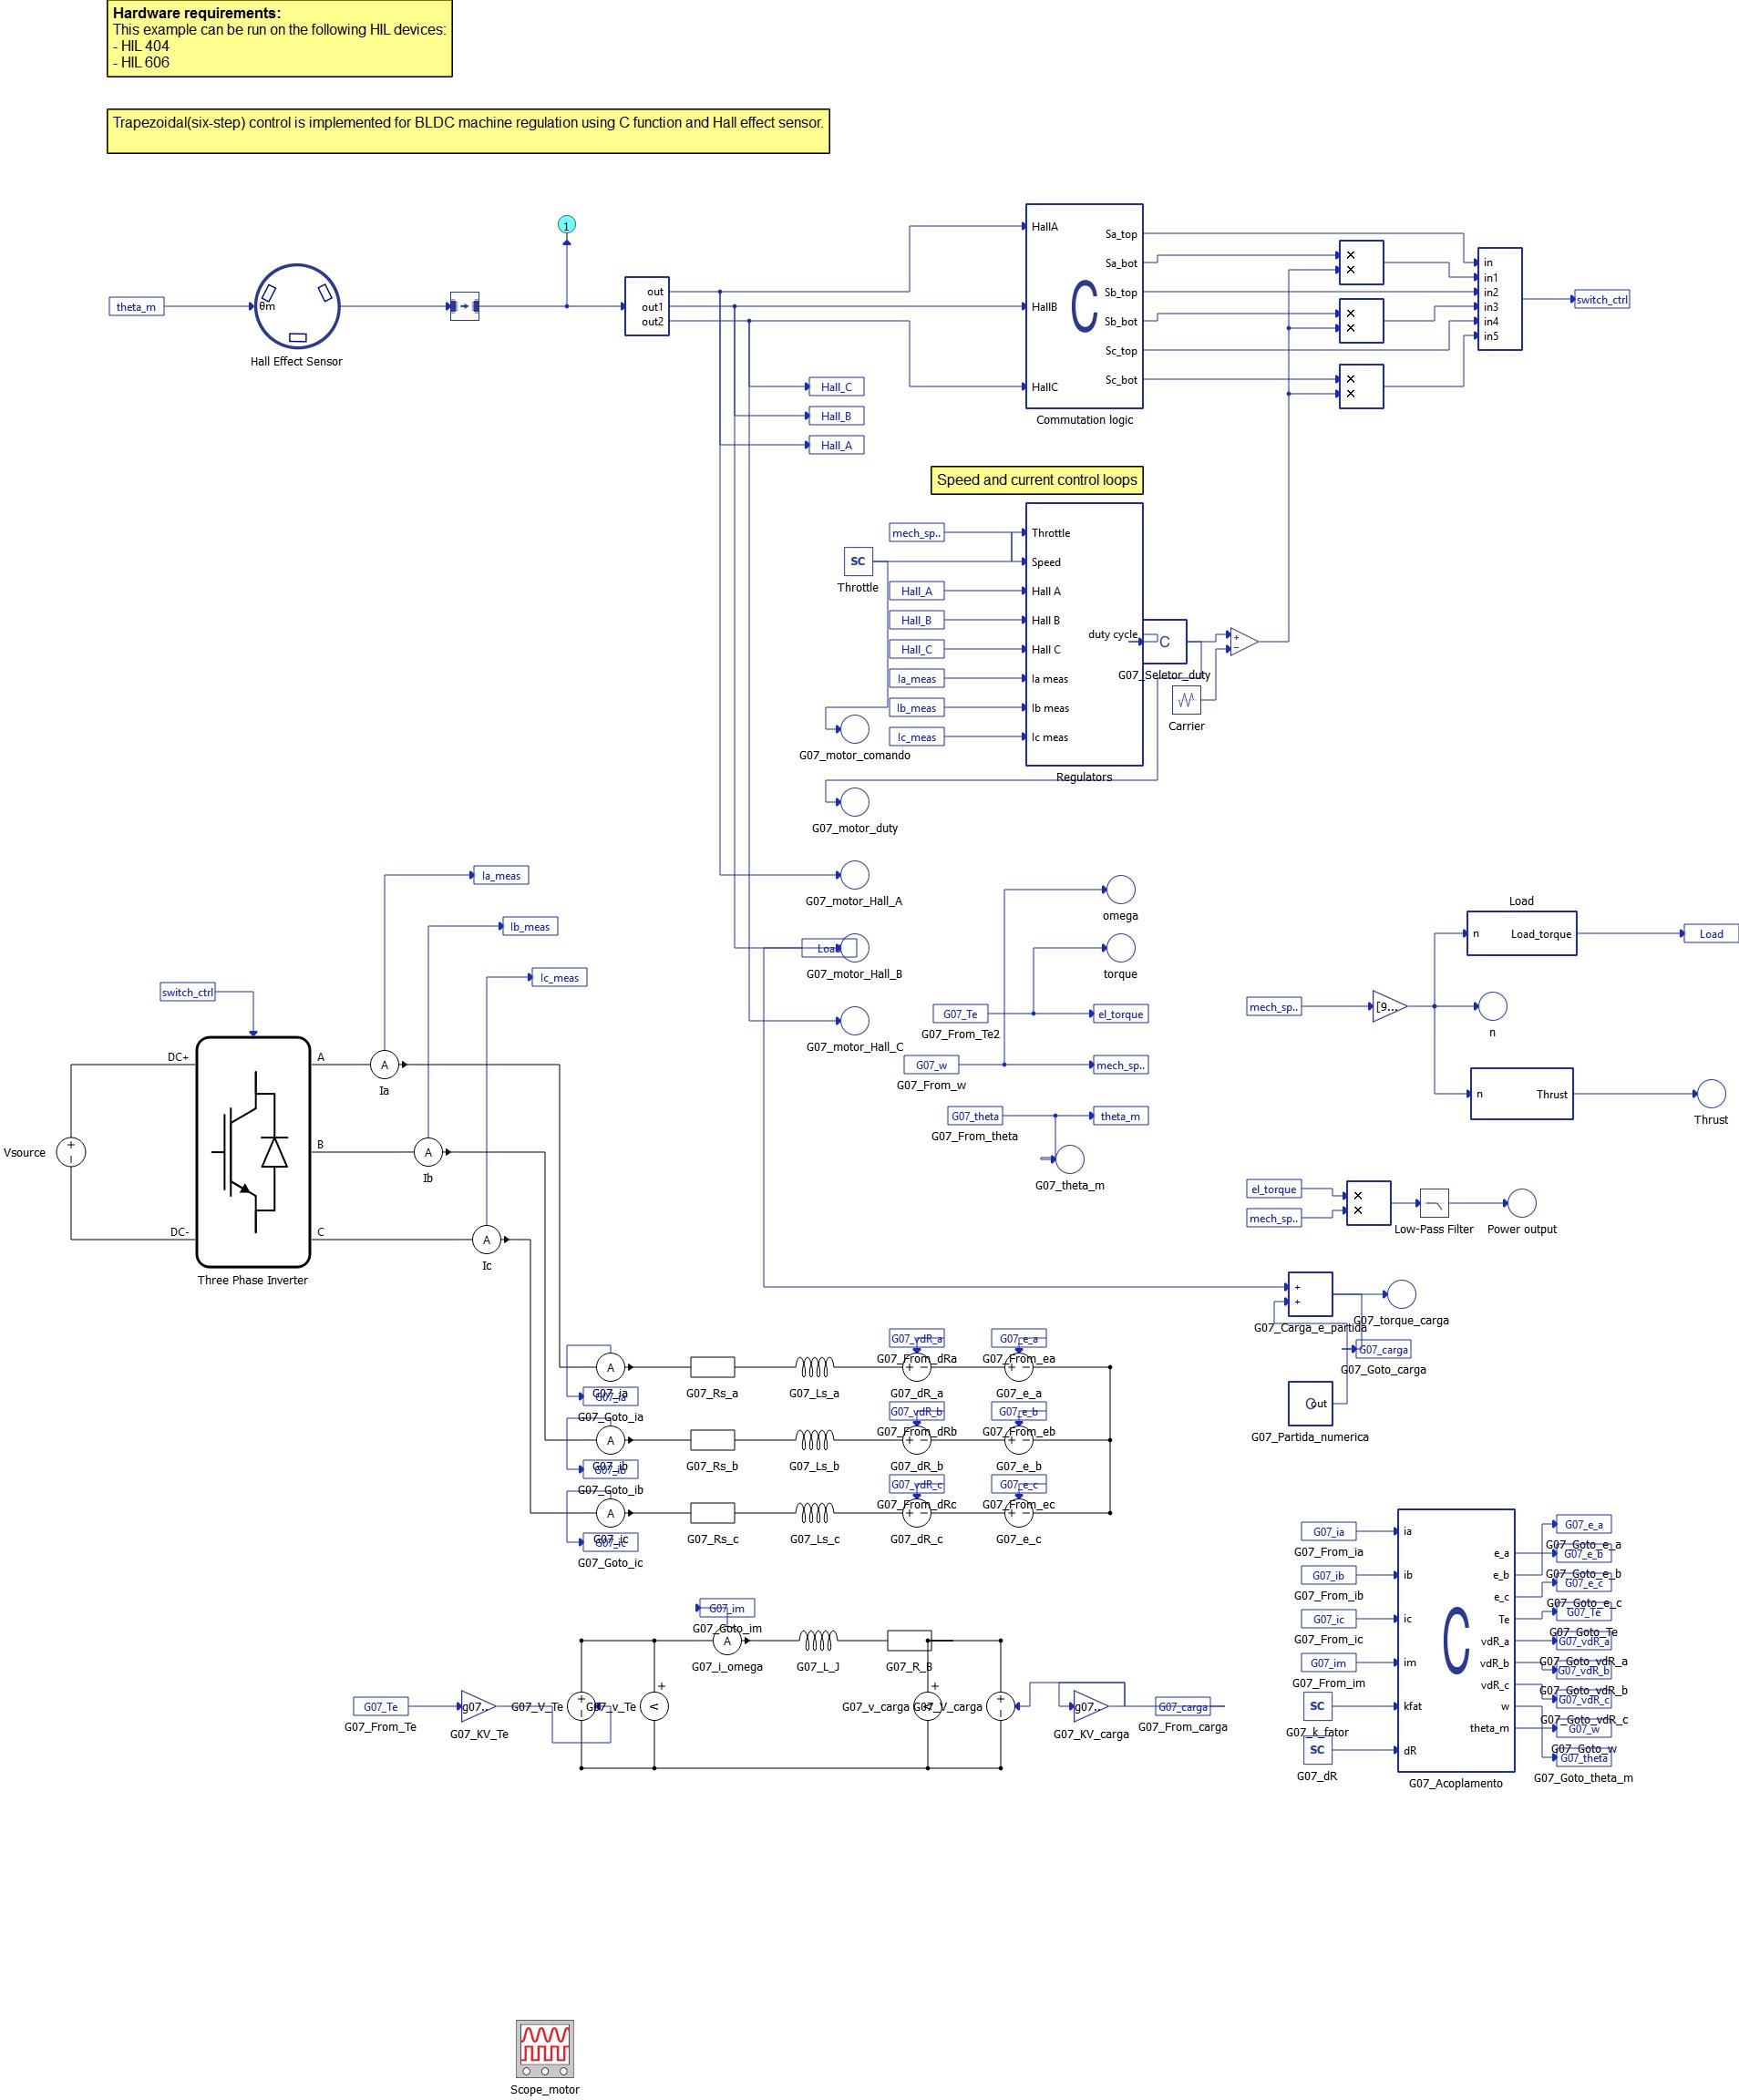
\includegraphics[width=0.8\textwidth]{figuras/foto_motor.jpg}
\caption{Sistema completo no Schematic Editor (\texttt{modelo\_equivalente.tse}): motor BLDC MOONS' R42BLD30L3 (42 mm, 36 V, 30 W, 8 polos, sensores Hall a 120° [2]; parâmetros na Tab.~1 da E01) com inversor, sensor Hall, lógica de comutação e malhas de controle da E01 (em cima) e, no lugar do bloco da máquina, as três fases equivalentes ($R_s$, $L_s$, $\Delta R\,i_x$, $e_x$), a malha mecânica ($L_J$, $R_B$, fontes de torque e carga) e a \texttt{C function} \texttt{G07\_Acoplamento} com as entradas de SCADA \texttt{G07\_k\_fator} e \texttt{G07\_dR} (embaixo).}\label{fig:foto}
\end{figure}

\R{Método de simulação}
O equivalente foi construído no Typhoon HIL Schematic Editor 2026.3 a partir do \texttt{.tse} da E01: o bloco \texttt{core/Brushless DC Machine} foi retirado e, no seu lugar, entrou o circuito da Fig.~\ref{fig:circ} (esquemático completo na Fig.~\ref{fig:foto}). Inversor, lógica Hall/comutação, PWM, malha de controle, carga e seletor de ensaio (\texttt{g07\_modo}) são os mesmos da E01, de modo que \emph{só a representação da planta muda}. Os componentes novos (prefixo \texttt{G07\_}) estão listados na Tab.~\ref{tab:inv}; os sinais entre o circuito e a \texttt{C function} passam por tags Goto/From, como no restante do modelo da E01.


\begin{table}[!htbp]\centering\small
\caption{Como cada resultado foi obtido.}\label{tab:metodo}
\begin{tabularx}{\textwidth}{p{3.3cm}p{3.2cm}Y}\toprule
Curva / origem & Modelo & Integração e amostragem\\\midrule
E01 modelo médio (só R1e) & reduzido de 3.ª ordem, Eq.~(3) da E01 & \texttt{solve\_ivp} DOP853, rtol = atol = $10^{-12}$\\
E01 trifásico (Python) & forma original, Eqs.~(1)–(2) da E01, inversor com diodos & Euler explícito, $\Delta t$ = 0,25 µs; Hall a 50 µs; portadora e comparador a $T_s$ = 5 µs (quantização de $d$ em 0,1)\\
E01 TyphoonSim (CSV) & \texttt{.tse} da E01 com o bloco BLDC & circuito: passo 2 µs, discretização exata; bloco BLDC a 50 µs; exportado do \texttt{Scope\_motor} a cada 10 ms\\
E02 equivalente & circuito da Fig.~\ref{fig:circ} (\texttt{modelo\_equivalente.tse}) & circuito: passo 2 µs (VHIL/TyphoonSim); \texttt{C function} de acoplamento a $10T_s$ = 50 µs (mesma taxa do bloco BLDC substituído); carga a 50 µs; PI de velocidade a 50 µs e de corrente a 25 µs. Curvas: \fonteEq{} (Euler 0,25 µs com as mesmas taxas de amostragem do \texttt{.tse}).\\\bottomrule
\end{tabularx}
\end{table}

\begin{figure}[!htbp]\centering
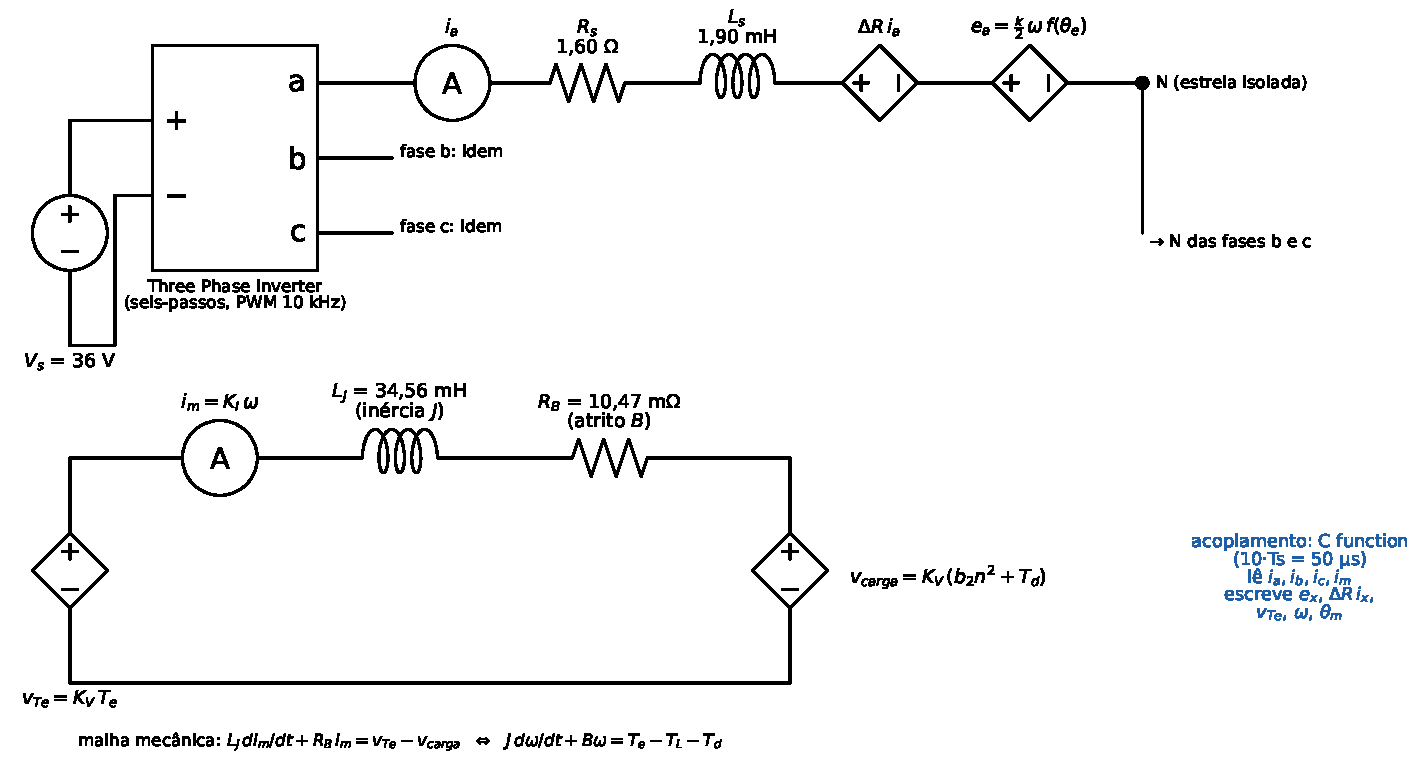
\includegraphics[width=\textwidth]{figuras/fig_circuito.pdf}
\caption{Circuito equivalente montado no TyphoonSim (fase $a$; $b$ e $c$ são iguais e se unem em N). Em cima, o lado elétrico na escala 1:1; embaixo, a malha mecânica pela analogia força–tensão. As fontes em losango são \texttt{core/Signal Controlled Voltage Source} (taxa $T_s\cdot10$); os amperímetros são \texttt{core/Current Measurement}.}\label{fig:circ}
\end{figure}

\R{R1. Analogia e escalonamento}
\textbf{(a) Correspondência.} A parte elétrica do motor já é um circuito e fica na escala 1:1. A parte mecânica usa a analogia força–tensão (impedância): esforço → tensão e fluxo → corrente, como no lado elétrico. Como $J$, $B$ e a carga compartilham a mesma velocidade, eles ficam \emph{em série} numa malha percorrida por $i_m\propto\omega$. O acoplamento eletromecânico ($e=k\omega$, $T_e=ki$) é um girador: cada lado é uma fonte controlada pela corrente do outro.

\begin{table}[!htbp]\centering\small
\caption{Correspondência entre o domínio eletromecânico e o circuito.}\label{tab:analog}
\begin{tabularx}{\textwidth}{p{3.6cm}p{2.6cm}p{4.2cm}Y}\toprule
Grandeza / elemento original & Papel & Par elétrico & Elemento no \texttt{.tse}\\\midrule
torque $T$ [N·m] & esforço & tensão $v=K_V T$ & --\\
velocidade $\omega$ [rad/s] & fluxo & corrente $i_m=K_I\omega$ & \texttt{G07\_i\_omega} (medidor)\\
inércia $J$ & armazena ($\tfrac12J\omega^2$) & indutor $L_J$ ($\tfrac12L_Ji_m^2$) & \texttt{G07\_L\_J}\\
atrito viscoso $B$ & dissipa ($B\omega^2$) & resistor $R_B$ & \texttt{G07\_R\_B}\\
carga $T_L=b_2n^2$ e pulso $T_d$ & dissipa / fonte & fonte de tensão controlada $v_{carga}$ & \texttt{G07\_V\_carga}\\
torque eletromagnético $T_e$ & fonte (girador) & fonte de tensão controlada $v_{Te}$ & \texttt{G07\_V\_Te}\\
FCEM $e_x=\tfrac k2\omega f(\theta_e-\varphi_x)$ & fonte (girador) & fonte de tensão controlada por $i_m$ & \texttt{G07\_e\_a/b/c}\\
$R_s$, $L_s$ de fase & dissipa / armazena & resistor e indutor (1:1) & \texttt{G07\_Rs\_x}, \texttt{G07\_Ls\_x}\\
corrente de fase $i_x$ & fluxo & corrente (1:1) & \texttt{G07\_ia/ib/ic}\\
$V_s$, inversor & fonte & os mesmos da E01 & \texttt{Vsource}, \texttt{Three Phase Inverter}\\
posição $\theta_m=\int\omega\,dt$ & não armazena energia & $\int i_m\,dt/K_I$ (envolta em $2\pi$) & saída \texttt{theta\_m} da \texttt{C function}\\\bottomrule
\end{tabularx}
\end{table}

\textbf{(b) Equações do circuito.} Lei das malhas em cada fase e na malha mecânica:
\begin{gather}
v_x-v_N=R_s i_x+L_s\frac{di_x}{dt}+\Delta R\,i_x+e_x,\qquad e_x=\frac k2\,\frac{i_m}{K_I}\,f(\theta_e-\varphi_x),\qquad i_a+i_b+i_c=0, \label{eq:fase}\\
L_J\frac{di_m}{dt}+R_B\,i_m=v_{Te}-v_{carga},\qquad v_{Te}=K_V\frac k2\sum_x f(\theta_e-\varphi_x)\,i_x,\qquad v_{carga}=K_V\,(b_2n^2+T_d),\qquad \frac{d\theta_m}{dt}=\frac{i_m}{K_I}. \label{eq:mec}
\end{gather}
Com $\Delta R=0$, (\ref{eq:fase}) é a Eq.~(1) da E01 com $\omega=i_m/K_I$. Substituindo $i_m=K_I\omega$, $L_J=JK_V/K_I$ e $R_B=BK_V/K_I$ em (\ref{eq:mec}) e dividindo por $K_V$: $J\dot\omega+B\omega=T_e-b_2n^2-T_d$, que é a Eq.~(2) da E01 (com $T_L=c\,\omega|\omega|$ e $\omega\ge0$ nos ensaios). As equações são, portanto, idênticas, termo a termo, após a conversão de escala. A potência na malha mecânica é $v_{Te}i_m=K_VK_I\,T_e\omega=0{,}955\,T_e\omega$: a escala quase preserva a potência.

\textbf{(c) Fatores de escala.} Escala de tempo 1:1 (o equivalente roda em tempo real no HIL, com 594 passos de 2 µs por $\tau_e$). Os fatores mantêm as grandezas da malha mecânica na mesma ordem das do lado elétrico (unidades de ampère, dezenas de volts), o que é bom para a precisão simples do \texttt{.tse} e para os sensores da Entrega 03, e têm leitura direta: 1 A = 1000 rpm e 1 V = 10 mN·m.
\begin{table}[!htbp]\centering\footnotesize
\caption{Escalas e faixas (domínio de validade da E01: $0\le n\le4500$ rpm, $|i|\le5$ A, $T\le0{,}24$ N·m).}\label{tab:escala}
\begin{tabular}{llll}\toprule
Variável & Fator & Faixa original & Faixa no circuito\\\midrule
$\omega$ → $i_m$ & $K_I=60/(2\pi\cdot1000)=9{,}5493\times10^{-3}$ A·s/rad & 0 a 471 rad/s (0 a 4500 rpm) & 0 a 4,5 A\\
$T_e$ → $v_{Te}$ & $K_V=100$ V/(N·m) & $-0{,}05$ a 0,24 N·m (pico de partida 0,23) & $-5$ a 24 V\\
$T_L+T_d$ → $v_{carga}$ & $K_V$ & 0 a 0,10 N·m (4500 rpm) + 0,02 & 0 a 12 V\\
$i_x$, $v_x$, $e_x$ & 1 & $|i|\le5$ A; $V_s$ = 36 V; $|e_x|\le11{,}3$ V & idem\\
tempo & 1 & $\tau_e$ = 1,19 ms; $\tau_m$ = 3 a 4,6 ms; $J/B$ = 3,3 s & idem\\\bottomrule
\end{tabular}
\end{table}

\textbf{(d) Parâmetros do circuito.}
$L_J=\dfrac{JK_V}{K_I}=\dfrac{3{,}3\times10^{-6}\cdot100}{9{,}5493\times10^{-3}}=34{,}558$ mH;\;
$R_B=\dfrac{BK_V}{K_I}=\dfrac{10^{-6}\cdot100}{9{,}5493\times10^{-3}}=10{,}472$ mΩ;\;
$R_s=1{,}60$ Ω e $L_s=1{,}90$ mH (1:1).
Ganhos das fontes controladas: FCEM $e_x=\frac{k}{2K_I}\,i_m f=2{,}513\,i_m f$ [V/A], isto é, $k/K_I=5{,}027$ V/A, o mesmo número do parâmetro \texttt{Emf} = 5,027 V/krpm da E01; torque $v_{Te}=K_V\frac k2\sum f i_x=2{,}4\sum f i_x$ [V/A]; carga $v_{carga}=K_Vb_2(1000\,i_m)^2=0{,}5\,i_m^2$ [V/A$^2$]; pulso $T_d$ = 0,02 N·m → 2 V. Conferência: $L_J/R_B=J/B=3{,}3$ s.

\textbf{(e) Verificação contra a R2 da E01.} Linearizando (\ref{eq:fase})–(\ref{eq:mec}) no modelo reduzido ($R_{LL}=2R_s$, $L_{LL}=2L_s$, $R_c=K_V(B+2c\omega_0)/K_I$), o circuito tem matriz $\begin{bmatrix}-R_{LL}/L_{LL}&-(k/K_I)/L_{LL}\\ K_Vk/L_J&-R_c/L_J\end{bmatrix}$, cujos autovalores, $\omega_n$, $\zeta$ e ganho estático (em A de $i_m$ por unidade de $d$, convertido por $1/K_I$) coincidem com os da Tab.~2 da E01 (Tab.~\ref{tab:lin}). $\tau_e=L_{LL}/R_{LL}$ = 1,1875 ms é o mesmo, porque o lado elétrico está em 1:1.
\begin{table}[!htbp]\centering\footnotesize\setlength{\tabcolsep}{4pt}
\caption{Circuito × E01 (R2) no repouso e em 4000 rpm. Pares ``a / b'': circuito / E01.}\label{tab:lin}
\begin{tabular}{lccccccc}\toprule
Ponto & $R_c$ [Ω] & polos (circuito) & polos (E01) & $\omega_n$ [rad/s] & $\zeta$ & $\tau_m$ [ms] & $G$: $i_m$ → rpm\\\midrule
\inputtab tabelas/tab_lin.tex \bottomrule
\end{tabular}
\end{table}

\R{R2. Implementação com a biblioteca nativa}
\begin{table}[!htbp]\centering\small
\caption{Inventário do \texttt{modelo\_equivalente.tse} (componentes novos; o restante é o acionamento da E01).}\label{tab:inv}
\begin{tabularx}{\textwidth}{p{3.4cm}p{4.6cm}p{2.6cm}Y}\toprule
Parte do modelo & Elemento nativo (biblioteca \texttt{core}) & Valor & Observação\\\midrule
$R_s$ de fase (×3) & \texttt{Resistor} & \texttt{Rs} = 1,60 Ω & \\
$L_s$ de fase (×3) & \texttt{Inductor} & \texttt{Ls} = 1,90 mH & neutro isolado: $L_s=L-M$\\
FCEM $e_x$ (×3) & \texttt{Signal Controlled Voltage Source} & da \texttt{C function} & 50 µs\\
$\Delta R\,i_x$ (×3, R4) & \texttt{Signal Controlled Voltage Source} & \texttt{G07\_dR}·$i_x$ & 0 no nominal\\
inércia $J$ & \texttt{Inductor} \texttt{G07\_L\_J} & \texttt{L\_J} = 34,56 mH & \\
atrito $B$ & \texttt{Resistor} \texttt{G07\_R\_B} & \texttt{R\_B} = 10,47 mΩ & \\
torque $T_e$ & \texttt{Signal Controlled Voltage Source} + \texttt{Gain} & $K_V$ = 100 & \texttt{G07\_V\_Te}, \texttt{G07\_KV\_Te}\\
carga $b_2n^2$, $T_d$, partida & \texttt{Signal Controlled Voltage Source} + \texttt{Gain}; subsistema \texttt{Load} (\texttt{Mathematical function}, \texttt{Gain}, \texttt{Sum}) & $b_2$ = $5\times10^{-9}$ & \texttt{Load} e \texttt{G07\_Partida\_numerica} vêm da E01\\
leitura de $\omega$, $i_x$ & \texttt{Current Measurement} & -- & \texttt{G07\_i\_omega}, \texttt{G07\_ia/ib/ic}\\
leitura de $T_e$, $T_L$ & \texttt{Voltage Measurement} & -- & \texttt{G07\_v\_Te}, \texttt{G07\_v\_carga}\\
parâmetros no SCADA & \texttt{SCADA Input} & 1 e 0 & \texttt{G07\_k\_fator}, \texttt{G07\_dR}\\
forma $f(\theta_e)$, $\theta_m$, produtos $\omega f$ e $\sum f i$ & \textbf{\texttt{C function} \texttt{G07\_Acoplamento}} (25 linhas) & $k/2$, $K_I$, $p$ & ver abaixo\\\bottomrule
\end{tabularx}
\end{table}
\textbf{Por que há uma \texttt{C function}.} A biblioteca não oferece fonte de FCEM trapezoidal nem girador como elementos de circuito: a única implementação nativa é o próprio bloco \texttt{Brushless DC Machine}, que é o que o equivalente substitui. A \texttt{C function} contém só o que falta: o trapézio $f(\cdot)$ com topo de 120°, os produtos $\frac k2\omega f$ e $\frac k2\sum fi_x$ e a integral $\theta_m=\int\omega\,dt$ envolta em $[0,2\pi)$, que evita o crescimento ilimitado do ângulo em precisão simples (o mesmo motivo da \texttt{C function} \texttt{rem} do subsistema Hall da E01). Todo armazenamento e dissipação de energia está nos R e L nativos, e as leituras são feitas por medidores ideais.

\R{R3. Validação contra o domínio original}
Foram repetidos os ensaios da E01: (a) degrau de $d$ a partir do repouso e (a$'$) degrau pequeno a partir do equilíbrio; (b) condição inicial não nula (4000 rpm em malha fechada e $d=0$ a partir de 150 ms); (c) pulso de carga $T_d$ = 0,02 N·m entre 100 e 200 ms, em malha aberta e fechada. Duas mudanças em relação à E01, ambas por causa da quantização do PWM do \texttt{.tse} ($d$ efetivo em passos de 0,1, R4 da E01): (a$'$) usa 0,867 → 0,95 ($d_{ef}$ 0,85 → 0,95), porque 0,867 → 0,887 não muda $d_{ef}$; e o ensaio fora do equilíbrio (b$'$) usa $d$ = 0,55, porque $d$ = 0,5 coincide com um degrau da portadora e o resultado passa a depender do arredondamento (1,6 \% de diferença entre implementações). Como o sistema é não linear, (a), (b) e (b$'$) validam longe do equilíbrio: partida com pico de 6,4 A, desaceleração de Riccati e condução descontínua.

\textbf{Execução em VHIL/SCADA.} Cada ensaio foi compilado para o Virtual HIL (HIL101) e capturado no HIL SCADA pelo \emph{Capture} do widget Capture/Scope: 0,3 s a 50 kS/s, sinais \texttt{n}, \texttt{torque}, \texttt{Ia}, \texttt{Ib}, \texttt{Ic}, \texttt{G07\_motor\_duty} e \texttt{G07\_v\_carga}, gatilho em \texttt{n} (borda de subida, 20 rpm, \emph{Use first trigger}) armado antes de iniciar a simulação. O tempo de cada captura é alinhado ao da simulação pelo evento do ensaio (degrau de \texttt{G07\_motor\_duty} em (a) e (a$'$), troca de $d$ em 150 ms em (b) e (b$'$), salto de 2 V de \texttt{G07\_v\_carga} em 100 ms em (c) e (c$'$)). Arquivos: \texttt{simulacao/dados-vhil-e2/vhil\_*.csv}.

\textbf{PWM em tempo real.} O modulador (portadora e comparador da E01, comum aos dois domínios e fora da planta) aplica no VHIL um $d$ efetivo um pouco diferente do TyphoonSim: 0,759 em vez de 0,75 no degrau (a), 0,841 → 0,959 em vez de 0,85 → 0,95 em (a$'$). Para comparar a \emph{planta}, o $d_{ef}$ de cada ensaio em malha aberta foi identificado pelo $n_{ss}$ do próprio VHIL, e o trifásico da E01 foi rodado com esse $d_{ef}$ (PWM ideal). Cada identificação usa um único número por ensaio (marcado na Tab.~\ref{tab:val}); tempos, picos, $\Delta n$, condução descontínua e os ensaios em malha fechada e de desaceleração livre são previsões independentes.

\textbf{Critério de concordância.} Grandezas de regime: $|\Delta|\le0{,}5$ \%, pouco acima da diferença TyphoonSim × Python da E01 (0,2 \%) e da ondulação de comutação (12 rpm p-p, 0,3 \%). Tempos de grandes sinais e $t_{1/2}$: $\le$ 5 \% e $\le$ 1 \%. Grandezas do degrau pequeno: $\le$ 10 \% para tempos e 2 \% para ganho, porque a ondulação (±6 rpm) já vale 2 \% de $\Delta n$ = 296 rpm e desloca o cruzamento de 90 \%. Pico de corrente e $\Delta n$: 2 \%.

\begin{figure}[!htbp]\centering
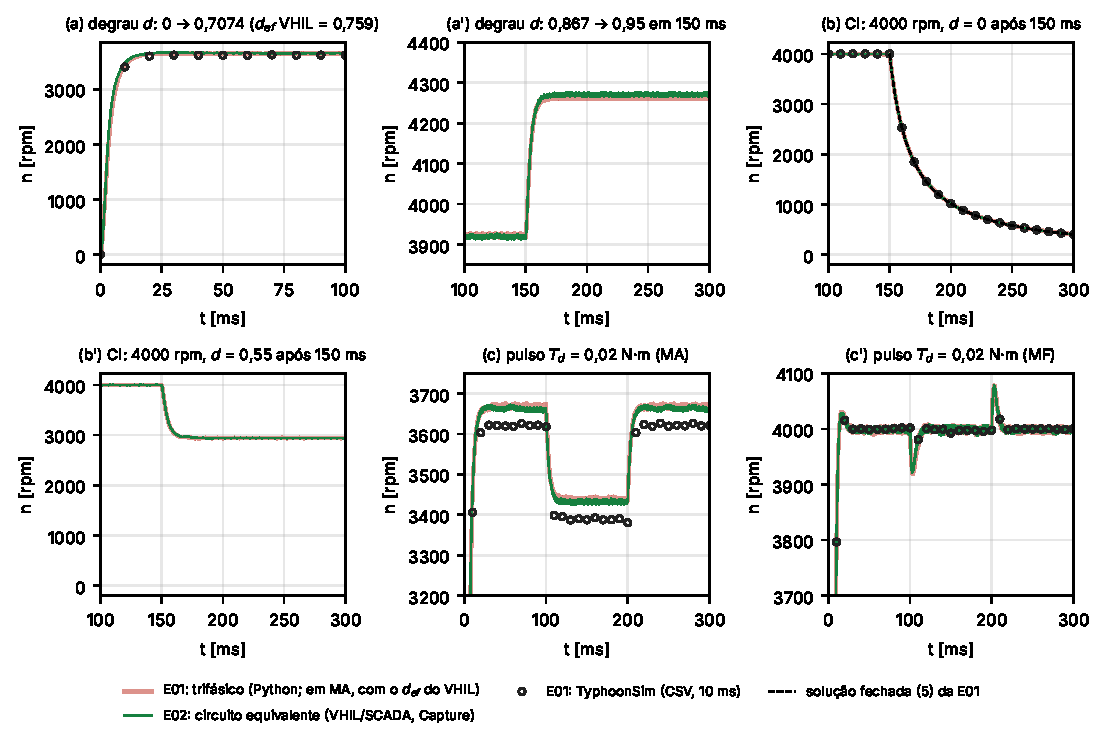
\includegraphics[width=\textwidth]{figuras/fig_validacao.pdf}
\caption{Equivalente executado no VHIL e capturado no HIL SCADA (verde; reconvertido: $n=1000\,i_m$) × E01 trifásico (vermelho; em malha aberta com o $d_{ef}$ identificado no VHIL) × CSV do TyphoonSim da E01 (círculos, $d_{ef}$ = 0,75, por isso abaixo em (a) e (c)). Tracejado em (b): solução fechada de Riccati (Eq.~5 da E01) a partir de 150 ms.}\label{fig:val}
\end{figure}

\begin{table}[!htbp]\centering\scriptsize
\caption{Grandezas características: equivalente no VHIL/SCADA (E02) × E01 trifásico nas mesmas condições × TyphoonSim da E01 (quando há CSV; $d_{ef}$ = 0,75). Diferença = (E02 − E01)/E01. Malha fechada original: TyphoonSim.}\label{tab:val}
\begin{tabularx}{\textwidth}{p{2.6cm}p{3.1cm}rrrrrY}\toprule
Ensaio & Grandeza & E02 & E01 & E01 Ty & Dif. [\%] & Crit. [\%] & Explicação\\\midrule
\inputtab tabelas/tab_validacao.tex \bottomrule
\end{tabularx}
\end{table}

\begin{figure}[!htbp]\centering
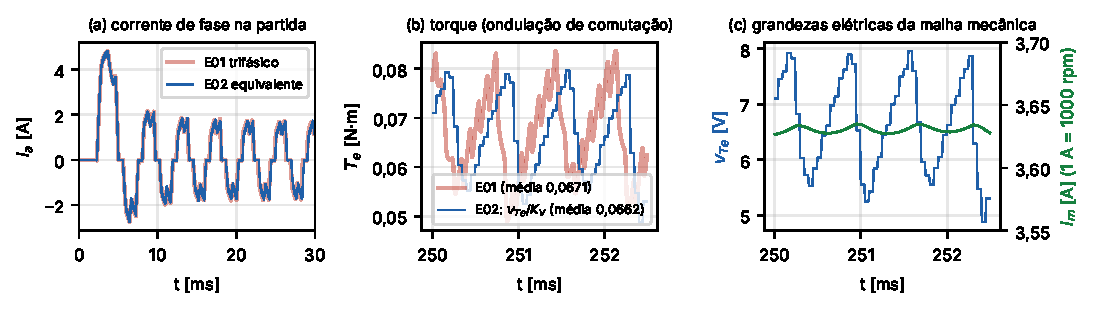
\includegraphics[width=\textwidth]{figuras/fig_correntes.pdf}
\caption{(a) Corrente de fase na partida; (b) torque em regime (degrau do repouso): mesma média, com ondulação de 0,031 N·m p-p no equivalente e 0,038 N·m no trifásico (amostragem de 50 µs); (c) $v_{Te}$ e $i_m$: o indutor $L_J$ filtra a ondulação de torque como a inércia.}\label{fig:corr}
\end{figure}

\textbf{Explicação das diferenças.} Dos 22 itens, 19 estão dentro do critério. A desaceleração livre (b), que não depende do PWM, concorda em até 0,17 \% e $t_{1/2}$ em 0,01 \%; o pulso em malha aberta dá $\Delta n$ com $-$0,8 \% e $t_{63}$ da queda igual; a malha fechada e o pulso em malha fechada concordam em 0,07 \% ou menos; a condução descontínua de (b$'$) termina 0,52 ms após a troca de $d$, contra 0,51 ms. Ficam fora: (i) $t_{63}$ e $t_s$ da partida (a), 7--8 \% mais rápidos no VHIL. O mesmo \texttt{.tse} no TyphoonSim dá $+$0,07 \% e $-$1,0 \% (E02 anterior, PWM quantizado), logo a diferença vem do modulador em tempo real na partida, quando o $d$ efetivo de cada período depende da fase da portadora, e não do circuito equivalente; (ii) o ganho incremental de (a$'$), $+$2,9 \%: o $\Delta d_{ef}$ = 0,118 vem de duas identificações, cada uma com incerteza de $\pm$1 rpm em 350 rpm, e a FCEM retida por 50 µs já dava $+$1,4 \% no TyphoonSim. Nos dois casos o comportamento qualitativo e as constantes de tempo do degrau pequeno ($-$3,5 \% e $+$2,8 \%) seguem a E01. A razão $T_e/|i|$ em regime vale 0,0475 N·m/A no equivalente, contra 0,0476 a 0,0479 no TyphoonSim da E01 e 0,048 nominal. No TyphoonSim, os mesmos sete ensaios (E02, \texttt{dados-typhoon-e2}) ficaram todos dentro do critério, com diferenças de regime entre 0,002 e 0,34 \%.

\R{R4. Sensibilidade no equivalente}
Parâmetros da R5 da E01: $k$ (pelo SCADA, \texttt{G07\_k\_fator}, que multiplica $k$ na FCEM e no torque) e $R_{LL}$ (pelo SCADA, \texttt{G07\_dR}, fonte $\Delta R\,i_x$ em série com cada fase; $R_{LL}=2(1{,}6+\Delta R)$). $J$ é um indutor e só muda recompilando ($L_J=JK_V/K_I$), por isso entra como verificação adicional. Ensaio: degrau do repouso.

\begin{figure}[!htbp]\centering
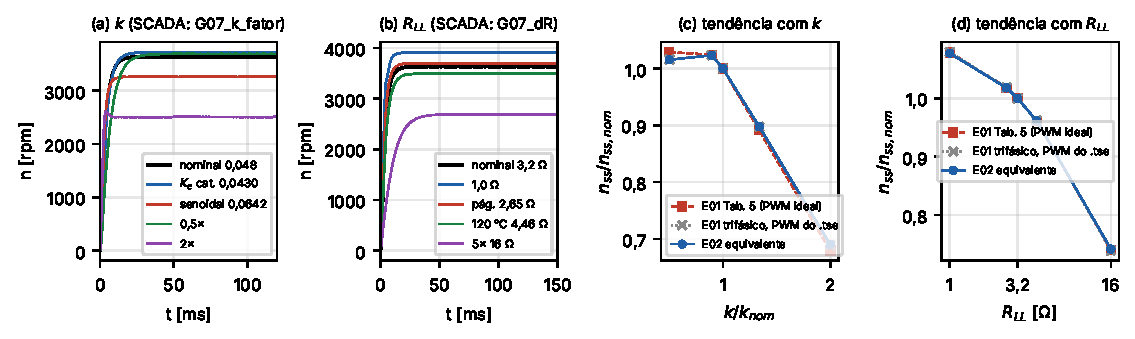
\includegraphics[width=\textwidth]{figuras/fig_sensibilidade.pdf}
\caption{(a), (b) $n(t)$ no equivalente para cada nível; (c), (d) tendência de $n_{ss}$ normalizada: Tab.~5 da E01 (forma original, PWM ideal), trifásico da E01 com o PWM do \texttt{.tse} e equivalente.}\label{fig:sens}
\end{figure}
\begin{table}[!htbp]\centering\scriptsize
\caption{Sensibilidade: $n_{ss}$ [rpm] / $t_s$ [ms]. A coluna da E01 Tab.~5 usa PWM ideal ($d$ = 0,7074); as duas seguintes usam o PWM do \texttt{.tse} ($d_{ef}$ = 0,75). Última coluna: $n_{ss}/n_{ss,nom}$ na E01 Tab.~5 / no equivalente.}\label{tab:sens}
\begin{tabular}{llllllc}\toprule
Par. & Nível & Ajuste no SCADA & E01 Tab. 5 & E01 trif. (PWM .tse) & E02 equivalente & razão E01 / E02\\\midrule
\inputtab tabelas/tab_sens.tex \bottomrule
\end{tabular}
\end{table}
\textbf{Conclusão.} O equivalente responde aos parâmetros como o sistema original. Com o mesmo PWM, $n_{ss}$ concorda com o trifásico da E01 em até 0,4 \% e $t_s$ em até 8,3 \% (o pior caso é $k$ = 2×, com $t_s$ = 6 ms). A tendência normalizada coincide com a Tab.~5 da E01 em até 1,6 \%. $k$ define o ganho estático, com máximo próximo do nominal: $k$ menor eleva $\xi$ e a perda de torque na comutação. $R$ diminui o ganho e torna a resposta mais lenta, e o efeito sobre $n_{ss}$ é metade do previsto pelo modelo reduzido. $J$ não altera $n_{ss}$ e escala $t_s$ (13,8 → 17,3 → 150 ms), como na E01.

\textbf{R4 no VHIL/SCADA.} Os mesmos ajustes foram feitos com o modelo rodando no Virtual HIL (HIL101), lidos após alguns segundos de simulação, pelas caixas \texttt{G07\_k\_fator} e \texttt{G07\_dR} do \texttt{painel\_equivalente.cus}, com leitura de $n$ no mostrador após o regime (Tab.~\ref{tab:vhil}). Por volta de 2,6 s de simulação o $d$ efetivo do modulador da E01 passa de $\approx$0,76 para $\approx$0,707 ($n$ cai de 3658 para 3458 rpm em um degrau), provavelmente por arredondamento do tempo da portadora em precisão simples; depois disso $d_{ef}\approx d$, e o nominal (3458 rpm) se compara com a Tab.~5 da E01 (PWM ideal, 3488 rpm, $-0{,}9$ \%). Por isso R4 usa razões $n_{ss}/n_{ss,nom}$ lidas no mesmo regime. As razões normalizadas concordam com a E01 em até 0,8 \%.
\begin{table}[!htbp]\centering\footnotesize
\caption{R4 executado no VHIL/SCADA: $n_{ss}$ [rpm] lido no painel e razão $n_{ss}/n_{ss,nom}$.}\label{tab:vhil}
\begin{tabular}{lllll}\toprule
Ajuste no SCADA & E01 Tab. 5 & E02 VHIL & razão E01 & razão VHIL\\\midrule
nominal ($k$ = 1, $\Delta R$ = 0) & 3488 & 3458 & 1,000 & 1,000\\
\texttt{G07\_k\_fator} = 0,896 & 3571 & 3570 & 1,024 & 1,032\\
\texttt{G07\_k\_fator} = 1,3375 & 3108 & 3068 & 0,891 & 0,887\\
\texttt{G07\_dR} = $-1{,}1$ ($R_{LL}$ 1,0 Ω) & 3757 & 3700 & 1,077 & 1,070\\
\texttt{G07\_dR} = 0,63 ($R_{LL}$ 4,46 Ω) & 3349 & 3319 & 0,960 & 0,960\\\bottomrule
\end{tabular}
\end{table}

\R{R5. Repetibilidade (roteiro)}
\begin{enumerate}
\item Instalar o Typhoon HIL Control Center \textbf{2026.3}. Arquivos: \texttt{modelo\_equivalente.tse} (modelo) e \texttt{painel\_equivalente.cus} (painel do HIL SCADA), na pasta \texttt{entregas/fase-2/e2-equivalente-eletrico/simulacao/} do repositório (branch \texttt{g07-motor-bldc}).
\item Abrir o arquivo no Schematic Editor, em \emph{View > Change perspective > TyphoonSim}. Em \emph{Model > Model settings > Model initialization}, escolher o ensaio pelas variáveis da Tab.~\ref{tab:roteiro} (\texttt{g07\_modo}, \texttt{g07\_d\_ini}, \texttt{g07\_d\_deg}, \texttt{g07\_t\_deg}, \texttt{g07\_d\_ci}).
\item Compilar e conferir no console: \texttt{L\_J=0.034558 H R\_B=0.010472 ohm}.
\item Simular 0,3 s (solver DAE/BDF, passo máximo 2 µs, já gravados no modelo) e ler no \texttt{Scope\_motor} os sinais \texttt{n}, \texttt{torque}, \texttt{Ia}, \texttt{Ib}, \texttt{Ic}, \texttt{G07\_v\_Te} e \texttt{G07\_v\_carga}. Exportar em CSV para registro. Conferências: $1000\cdot$\texttt{G07\_i\_omega} = \texttt{n} e \texttt{G07\_v\_Te}/100 = \texttt{torque}.
\item VHIL/SCADA: trocar para a perspectiva de tempo real (a malha mecânica já está referenciada ao neutro N pela conexão \texttt{G07\_E2\_ref}, necessária para que as fontes controladas sejam alocadas no HIL), compilar para o Virtual HIL e abrir o HIL SCADA com o modelo carregado e \emph{Virtual HIL} marcado. Abrir o painel \texttt{painel\_equivalente.cus} (mesma pasta), que já traz as entradas \texttt{G07\_k\_fator} (1) e \texttt{G07\_dR} (0) e os mostradores de \texttt{n}, \texttt{torque}, duty e $i_a$.
\item R3 no VHIL: para cada ensaio, ajustar as variáveis da Tab.~\ref{tab:roteiro} (manter \texttt{g07\_Td = 0.02}), compilar em tempo real e fazer \emph{Model > Reload Model} no SCADA. No Capture/Scope (modo \emph{Capture}): \emph{Time interval} 0,30 s, \emph{Sample rate} 50 KSPS, sinais \texttt{n}, \texttt{torque}, \texttt{Ia}, \texttt{Ib}, \texttt{Ic}, \texttt{G07\_motor\_duty}, \texttt{G07\_v\_carga}; gatilho \emph{Analog}, \texttt{n}, \emph{Rising edge}, 20, offset 5 \%, \emph{Use first trigger} marcado. Com a simulação parada, clicar no botão de captura com gatilho (\textbf{T}) e depois em \emph{Start simulation}; exportar em CSV (\emph{Save data}).
\item R4: com o modelo nominal rodando há alguns segundos, alterar \texttt{G07\_k\_fator} e \texttt{G07\_dR} no painel (valores da Tab.~\ref{tab:vhil}) e ler $n_{ss}$ no mostrador.
\item Resultado esperado: os valores da Tab.~\ref{tab:roteiro}, com tolerância igual ao critério de R3.
\end{enumerate}
\begin{table}[!htbp]\centering\footnotesize
\caption{Valores a ajustar e resultado esperado em cada ensaio (degrau = \texttt{g07\_modo} 1).}\label{tab:roteiro}
\begin{tabularx}{\textwidth}{p{2.6cm}Yp{5.6cm}}\toprule
Ensaio & Variáveis / SCADA & Resultado esperado\\\midrule
(a) degrau do repouso & \texttt{g07\_modo=1}, \texttt{g07\_d\_ini=0}, \texttt{g07\_d\_deg=0.7074}, \texttt{g07\_t\_deg=0} & $n_{ss}\approx$ 3658 rpm (VHIL) / 3623 (TyphoonSim), $t_s\approx$ 13--14 ms, $i_{pk}\approx$ 6,4 A\\
(a$'$) degrau pequeno & \texttt{g07\_modo=1}, \texttt{0.867} → \texttt{0.95} em \texttt{0.15} & 3919 → 4270 rpm (VHIL), $t_{63}\approx$ 4 ms\\
(b) CI, $d=0$ & \texttt{g07\_modo=2}, \texttt{g07\_d\_ci=0} & 2534 / 1849 / 1019 rpm em 0,16 / 0,17 / 0,20 s\\
(b$'$) CI, $d=0{,}55$ & \texttt{g07\_modo=2}, \texttt{g07\_d\_ci=0.55} & $n_{ss}\approx$ 2941 rpm (VHIL) / 2900 (TyphoonSim)\\
(c) pulso MA & \texttt{g07\_modo=3} & 3661 → 3431 rpm ($\Delta n\approx-230$, VHIL)\\
(c$'$) pulso MF & \texttt{g07\_modo=4} & $\approx$ 4000 rpm, mínimo $\approx$ 3922 rpm\\
malha fechada & \texttt{g07\_modo=0} & $\approx$ 3998 rpm\\
R4, $k$ (VHIL) & \texttt{G07\_k\_fator} = 0,896 / 1,3375 & $\approx$ 3570 / 3068 rpm (nominal $\approx$ 3458)\\
R4, $R$ (VHIL) & \texttt{G07\_dR} = $-1{,}1$ / 0,63 & $\approx$ 3700 / 3319 rpm\\\bottomrule
\end{tabularx}
\end{table}

\FloatBarrier

\section*{Apêndice A. Código externo: \texttt{C function} \texttt{G07\_Acoplamento}}
Único código externo do modelo (está dentro do \texttt{.tse}; não há arquivo separado). Entradas: $i_a,i_b,i_c$, $i_m$ (corrente da malha mecânica, $=K_I\omega$), \texttt{kfat} e \texttt{dR} (SCADA). Parâmetros (de \emph{Model initialization}): \texttt{g07\_kph} $=k/2$, \texttt{g07\_KI} $=K_I$, \texttt{g07\_Tc} $=10T_s$, \texttt{g07\_p} = pares de polos. Saídas: FCEM $e_x$, torque $T_e$ (vira $v_{Te}=K_VT_e$ fora do bloco), quedas $\Delta R\,i_x$, $\omega$ e $\theta_m$. O bloco só faz o que a biblioteca não oferece: a forma trapezoidal $f(\theta_e)$ e o girador; todo armazenamento e dissipação ficam nos R e L nativos.
{\scriptsize\VerbatimInput[frame=single,numbers=left,numbersep=3pt]{tabelas/codigo_c.txt}}

\begin{thebibliography}{9}\small
\bibitem{dossie} ECOM060. Banco de Sistemas: dossiê oficial do Motor BLDC (MOONS' R42BLD30L3). UFAL, 2026.
\bibitem{moons} MOONS'. BLDC Motors — catálogo, série R42BL. Disponível em: \url{https://shop.mev-elektronik.com/wp-content/uploads/MOONS_BLDC_Motors.pdf}.
\bibitem{e01} G07. Caracterização da planta no domínio de origem: motor BLDC MOONS' R42BLD30L3 (Fase 2, Entrega 01). ECOM060, UFAL, 2026.
\bibitem{ty} Typhoon HIL. Schematic Editor, HIL API e SCADA API — documentação da versão 2026.3 (instalada com o Control Center).
\bibitem{ogata} K. Ogata. \emph{System Dynamics}, 4.ª ed. Pearson, 2004 (analogias eletromecânicas).
\end{thebibliography}
\end{document}
